\chapter{Numerical Experiments}
\label{cha:3}
In this chapter we shall compare the augmented Lagrangian Method with several industry standard backpropagation algorithms. We considered the following algorithms: ADAM, ...

The first comparison will be run on a small example, for which we expect that all algorithms should easily converge to a good solution.

\section{Training Algorithms and Stopping Criteria}
This section will discuss the problem of comparing different training algorithms, which is not as straightforward as it might seem. In the literature many different methods of comparison are used, usually picking the one which fits their algorithm the best. The main issue is the choice of stopping criterion. One can choose a tolerance for the loss function, but this might not always be reached due to local minima. A second option is to stop after a set number of epochs, but an epoch in one algorithm is not necessarily equivalent to an epoch in another algorithm. A third option is to let each algorithm run for a specified length of time, and compare the loss on the training set after each run. This might be the most fair option, because average running time is the most important factor in practice. On the other hand it is hard for a new, experimental method to be as optimally coded as one that has been used in the field for many years already.

Further complicating the matter is that in practice many different early stopping criteria are used as well, to protect against overfitting. The most common early stopping criterion is to stop when a minimum in the validation dataset has been reached. Furthermore, because of the complexity of the loss surface of a DNN, and the random initialization of the weight matrices, each training run will follow a different trajectory and find a different local minimum.

Because the goal of this thesis is to compare training performance, overfitting is not a great concern. Therefore validation data will not be used in the training process. Instead the training will stop once the improvement in training loss stagnates, indicating a local minimum has been reached. ALM will stop when the following inequality holds true:

\begin{equation}
(1+\epsilon)C(W_{k+1}) > C(W_k)
\end{equation}
Where $C(W_k)$ is the loss at epoch $k$ and $\epsilon$ is a small tolerance value. Because ALM only takes only a few costly epochs to converge, it should make sense to not wait many epochs to confirm that the method has stagnated its progress. On the other hand the main algorithm against which the ALM method will be compared is the ADAM algorithm, which may take thousands of epochs to converge. To find the minimum in the training loss the \texttt{EarlyStopping} method implemented in \texttt{keras} will be used. This method has a patience value $p$, meaning that the training will stop once $p$ epochs have passed without any improvement.
 

\section{Test setup}
Each test will average the results over many training runs so as to get a more accurate and fair picture of the performance that can be expected from each algorithm. Typically each test will use 20 training runs.

The weights of the network will be initialized using Xavier initialization for the layers using the $\tanh(x)$ activation function and Kaiming initialization for the layers using the ReLU activation function, as is standard in practice. Both algorithms will start with the same initalization in each comparison.

All tests are run on .... , GBS,

\section{Fully connected feedforward network}
For the first comparison a similar regression problem as in chapter one will be considered. In a first try the same sine function was used as in equation \ref{} in chapter 1. The issue with this function is that it is too simple of a training problem. Both algorithms converge quite quickly to a very good solution, one of which is shown in figure \ref{}, and it is difficult to differentiate the algorithms. 

For this reason a problem with more depth is required. In this first test a squared sine function will be approximated instead. This function oscillates progressively faster, so that the training algorithm can always keep finding a better solution. Figure \ref{} shows how different training configurations let a network approximate a larger or smaller segment of the function. The function definition is as follows:

\begin{equation}
y = \sin^2(x) + \mathcal N(0,\delta), x \in [0,\pi]
\end{equation}

\begin{figure}
         \centering
         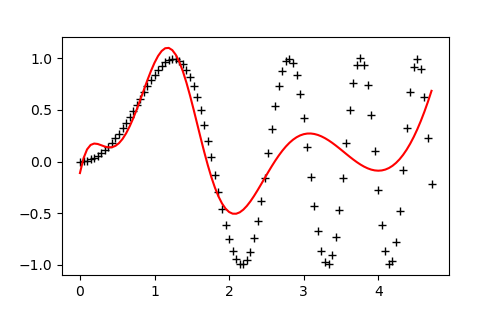
\includegraphics[width=\textwidth]{sine_squared}
         \caption{Feedforward network with 2 hidden layers of 20 relu units, trained on test function using ALM, using 80 training pairs}
\end{figure}

The training performance of the ALM method will be compared to the Stochastic Gradient Descent (SGD) method implemented in \texttt{keras}. The weights of the network will be initialized using Xavier initialization for the layers using the $\tanh(x)$ activation function and Kaiming initialization for the layers using the ReLU activation function. Both training algorithms will start from the same initial point for each test. Training will stop when progress on the training loss stagnates, indicating a local minimum has been reached. For SGD the \texttt{EarlyStopping} class will be used to stop the training when 4 epochs have passed without improvement, while for ALM the following stopping criterion will be used:

\begin{equation}
(1+\epsilon)C(W_{k+1}) > C(W_k)
\end{equation}
Where $C(W_k)$ is the loss at epoch $k$ and $\epsilon$ is chosen to be $1e^{-2}$.

In the first test the effect of the number of datapoints is analyzed, by taking a neural network

sine regression






\begin{itemize}
\item sine regression

	\item compare until validation performance under ...
	\item relu vs tanh
	\item depth of network
	\item width of network
	\item number of input-output pairs
	\item scalability
	
	
	
\begin{itemize}
	\item Optimization for deep learning: theory and algorithms
	\item Goals of optimization
	\item Problem formulation
	\item Gradient descent:
	\item Tips  tricks
	\item State of the art algorithms
\end{itemize}







\item
\cite{sun2019optimization}
\begin{itemize}
	\item Optimization for deep learning: theory and algorithms
	\item Goals of optimization
	\item Problem formulation
	\item Gradient descent:
	\item Tips  tricks
	\item State of the art algorithms
\end{itemize}


\item
\cite{dreyfus1990}

"The Kelley-Bryson gradient
formulas for such problems have been rediscovered by neural-
network researchers and termed back propagation"

\item
\cite{Birgin2009}

Practical Augmented lagrangian method

\item
\cite{jacot2020neural}
"Indeed
the loss surface of neural networks optimization problems is highly non-convex: it has a high number
of saddle points which may slow down the convergence (4). A number of results (3; 13; 14) suggest
that for wide enough networks, there are very few "bad" local minima, i.e. local minima with much
higher cost than the global minimum"
\item
\cite{Rumelhart1986}
Original Backpropagation paper


\end{itemize}

\section{Needed}

\begin{itemize}
\item
Basic Neural network intro

\item
Optimal control 

\item
Simultaneous approach
\end{itemize}



%%% Local Variables: 
%%% mode: latex
%%% TeX-master: "thesis"
%%% End: 
